\documentclass{exam}
\usepackage[russian, english]{babel}
\usepackage[T2A]{fontenc}
\usepackage[utf8]{inputenc}
\usepackage{graphicx}
\usepackage{amsmath}
\usepackage{comment}
\begin{document}

\begin{questions}
\section{Билет}
	\question 
		Стили программирования
	\question 
Для следующей системы найдите частоту \(\omega_m\), 
для которой величина усиления наибольшая.
	\[	
		\frac{1}{1+s+s^2}
		\]
\end{questions}
\vspace{15pt}

\newpage
\begin{questions}
\section{Билет}
	\question 
		Автоматы
	\question
Колеса прикреплены к автомобилю через систему подвески, 
предназначенную для минимизации вибраций салона, возникающих 
при движении по неровной местности.
Система подвески состоит из пружины и амортизатора, которые 
сжимаются при проезде колеса по неровностям, поэтому резкое 
движение колеса не передается напрямую в салон.
Пружина создает силу, удерживающую салон на нужном расстоянии 
от поверхности дороги, а амортизатор добавляет фрикционное демпфирование.
В этой задаче вы определите, какое демпфирование желательно, 
проанализировав простую модель системы подвески автомобиля, показанную ниже.


	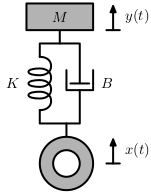
\includegraphics[width=8cm]{~/students/cs204.github.io/psets/data/images/frequency_response/car.png}

Модель состоит из массы M, которая представляет массу автомобиля, 
которая соединена с колесом через пружину и амортизатор.
Вертикальное смещение колеса от его положения равновесия принимается 
в качестве входных данных x(t).
Вертикальное смещение массы из положения равновесия принимается за выходной сигнал y(t).
Предполагается, что пружина подчиняется закону Гука, так что создаваемая 
ею сила равна константе, умноженной на величину сжатия пружины относительно 
ее равновесного сжатия.
Предполагается, что амортизатор создает силу, которая является постоянной 
величиной, умноженной на скорость, с которой амортизатор сжимается.
Обратите внимание, что, относя x(t) и y(t) к их положениям равновесия, 
силой гравитации можно пренебречь.
Предположим, что M = 1 и K = 1.
	
Определите дифференциальное уравнение, связывающее входной 
		сигнал x(t) и выходной сигнал y(t).

Определите и постройте импульсную характеристику системы, когда B = 0.
На основе этого результата дайте физическое объяснение проблемы, 
которая возникла бы, если бы в системе не было амортизатора.
	
\end{questions}

\newpage
\begin{questions}
\section{Билет}
	\question 
	Сигналы и системы 
	\question 
Отклик на импульс CT системы имеет вид

\[
h(t)=e^{-\sigma t} \cos(\omega_dt+\phi)u(t)
\]

где параметры \(\sigma\), \(\omega_d\) и \(\phi\) связаны с параметрами 
характеристического полинома системы: \(s^2 + Bs + C\).

Определите выражения для \(\sigma\) и \(\omega_d\)  
(не \(\phi\))  через B и C.

\end{questions}
\vspace{15pt}


\newpage
\begin{questions}
\section{Билет}
	\question 
Обратная связь, полюса и моды 

	\question 
Колеса прикреплены к автомобилю через систему подвески, 
предназначенную для минимизации вибраций салона, возникающих 
при движении по неровной местности.
Система подвески состоит из пружины и амортизатора, которые 
сжимаются при проезде колеса по неровностям, поэтому резкое 
движение колеса не передается напрямую в салон.
Пружина создает силу, удерживающую салон на нужном расстоянии 
от поверхности дороги, а амортизатор добавляет фрикционное демпфирование.
В этой задаче вы определите, какое демпфирование желательно, 
проанализировав простую модель системы подвески автомобиля, показанную ниже.


	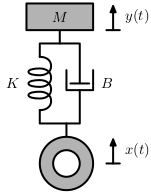
\includegraphics[width=8cm]{~/students/cs204.github.io/psets/data/images/frequency_response/car.png}

Модель состоит из массы M, которая представляет массу автомобиля, 
которая соединена с колесом через пружину и амортизатор.
Вертикальное смещение колеса от его положения равновесия принимается 
в качестве входных данных x(t).
Вертикальное смещение массы из положения равновесия принимается за выходной сигнал y(t).
Предполагается, что пружина подчиняется закону Гука, так что создаваемая 
ею сила равна константе, умноженной на величину сжатия пружины относительно 
ее равновесного сжатия.
Предполагается, что амортизатор создает силу, которая является постоянной 
величиной, умноженной на скорость, с которой амортизатор сжимается.
Обратите внимание, что, относя x(t) и y(t) к их положениям равновесия, 
силой гравитации можно пренебречь.
Предположим, что M = 1 и K = 1.
	
Определите выражение для наименьшей положительной 
		постоянной затухания B, при которой полюса системы имеют 
		действительные значения.  
		Нарисуйте импульсную характеристику системы для этого значения B.  
		На основе этого результата дайте физическое объяснение тому, 
		как амортизатор улучшает работу системы подвески.
\end{questions}
\vspace{15pt}



\newpage
\begin{questions}
\section{Билет}
	\question 
Непрерывные системы 
	\question 
Расширьте метод линейной интерполяции на два измерения.  
Напишите программу, которая использует этот метод для 
увеличения следующего изображения с его текущих размеров 
(212 × 216) в три раза.  
Сравните результат линейной интерполяции с результатом 
повторения каждого значения пикселя 3×3 раза (см. приложение).


Цифровая форма этого изображения доступна 
на 

	https://cs204.github.io/psets/data/images/convolution/zebra.jpg
\end{questions}
\vspace{15pt}

\newpage
\begin{questions}
\section{Билет}
	\question 
z-преобразования 
	\question 
Улыбка
Рассмотрим последовательность единиц и -1, показанную ниже как x[n].
 
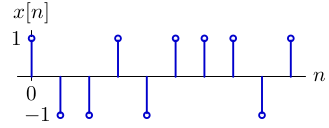
\includegraphics[width=8cm]{~/students/cs204.github.io/psets/data/images/convolution/smiley_x_n.png}

	В этом \(x[n]\) имеет единственное вхождение шаблона -1, -1, 1.
Это происходит начиная с n = 1 и заканчивая n = 3.
Один из методов автоматического обнаружения определённых шаблонов 
этого типа называется «согласованной фильтрацией».
Пусть p[n] представляет интересующий шаблон, перевёрнутый вокруг n = 0.
Тогда экземпляры шаблона можно найти, определив моменты 
времени, когда y[n] = (p * x)[n] максимизируется.

Определите согласованный фильтр p[n], который будет 
находить вхождения последовательности: -1, -1, 1.

Спроектируйте \(p[n]\) так, чтобы \((p*x)[n]\) имело максимумы в 
	точках, центрированных на желаемом шаблоне, т. е. в точке \( n = 2\) 
для приведённой выше последовательности.

Тот же подход можно использовать для поиска шаблонов на изображениях 
путём обобщения оператора свёртки на два измерения:


	\[
y[n,m]=(x*p)[n,m]=\sum_{k=-\infty}^\infty \sum_{l=-\infty}^\infty x[k,l]p[n-k, m-l].
\]

Файл 

	psets/data/images/convolution/findsmiley.jpg
содержит случайный набор белых пикселей (код 255) и чёрных пикселей (0), 
а также один экземпляр следующего смайлика:

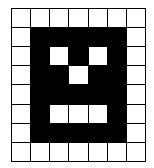
\includegraphics[width=4cm]{~/students/cs204.github.io/psets/data/images/convolution/smiley.png} 

Найдите строку и столбец findsmiley, соответствующий носу смайлика.
Примечание. Согласованная фильтрация будет работать лучше всего, 
если совпадение белых пикселей И совпадение чёрных пикселей 
положительно повлияют на ответ.
По этой причине 255 и 0 могут быть не оптимальным выбором для значений, 
связанных с белыми и чёрными пикселями.

\end{questions}
\vspace{15pt}



\newpage
\section{Билет}
\begin{questions}
	\question 
Преобразование Лапласа 
	\question 
На следующем рисунке показана каскадная система 
из двух резервуаров для воды. Вода течёт
	\begin{itemize}
		\item в первый бак скорость \(r_0(t)\),
		\item из первого бака и во второй скорость \(r_1(t)\),
		\item скорость вытекания из второго \(r_2(t)\).
	\end{itemize}

	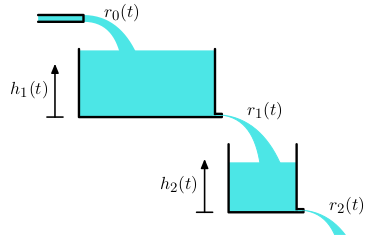
\includegraphics[width=8cm]{~/students/cs204.github.io/psets/data/images/leaky_tanks.png}

Скорость потока из каждого резервуара пропорциональна 
высоте воды в этом резервуаре:
	\[
\begin{split}
r_1(t)&=k_1h_1(t),\\
r_2(t)&=k_2h_2(t),\\
\end{split}
\]
где \(k_1\) и \(k_2\) каждый 0.2 метра2/секунду.
Оба резервуара имеют высоту 1 м. 
Площадь поперечного сечения резервуара 1 \(A_1 = 4 м^2\), 
второго резервуара \(A_2 = 2 м^2\).
В момент времени t = 0 оба резервуара пусты.

Пусть \(x(t) = r_0 (t)\) представляет собой вход 
резервуарной системы, а \(y(t) = r_2 (t)\) представляет выход.
Определите связь между входом и выходом.
Выразите это соотношение в виде дифференциального уравнения вида
	\[
a_0y(t)+a_1\frac{dy(t)}{dt}+a_2\frac{d^2y(t)}{dt^2}+...=x(t)+b_1\frac{dx(t)}{dt}+b_2\frac{d^2x(t)}{dt^2}+...
\]
где \(x(t)=1\).



Используйте приближение Эйлера вперёд для создания 
дискретной аппроксимации дифференциального соотношения 
между \(r_1 (t)\) и \(r_0 (t)\) следующим образом.
Пусть \(r_0(t)\) и \(r_1 (t)\) аппроксимируются 
дискретными последовательностями \(r_0 [n] = r_0 (nT)\) 
и \(r_1 [n] = r_1 (nT)\), где T представляет собой размер шага.
Затем аппроксимируем производную по непрерывному времени 
в момент времени nT первой разностью:
	\[
\left. \frac{dr_1(t)}{dt}\right\vert_{t=nT}\approx \frac{r_1[n+1]-r_1[n]}{T}
\]
Решите это разностное уравнение для \(r_1 [n + 1]\) через 
значения \(r_1 [k]\) и \(r0 [k]\), где k < n + 1, 
и введите результат ниже.


Используйте Python, чтобы решить эту рекурсию для особого случая, 
когда входное значение \(r_0 [n]\) поддерживается постоянным 
на уровне \(0.1 м3/с\), резервуар 1 изначально пуст и
T = 1 секунда (см. пример кода в поле ниже).
Постройте график вашего решения для 0 < t < 60.
Также отобразите аналитический результат из части c на тех же осях.
Определите максимальную разницу между аналитическими и численными результатами.

\end{questions}
\vspace{15pt}



\newpage
\section{Билет}
\begin{questions}
	\question 
Дискретная аппроксимация непрерывных систем 
	\question 
На следующем рисунке показана система - масса на пружинке.
Входные данные x(t) представляют положение верхнего конца пружины.
Выходные данные y(t) представляют положение массы.

	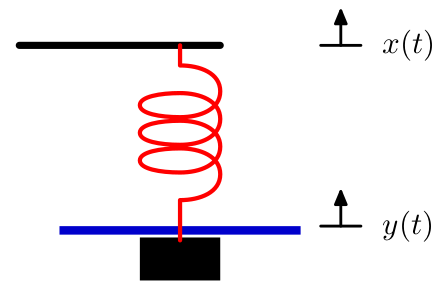
\includegraphics[width=8cm]{~/students/cs204.github.io/psets/data/images/spring.png}

Масса M = 1 кг, жёсткость пружины K = 1 Н/м.
Предположим, что пружина подчиняется закону Гука и что исходное 
положения определено так, что если входной сигнал x(t) равен нулю, 
то положение покоя y(t) также равно нулю.


		Определите дифференциальное уравнение, связывающее входной сигнал x(t) и выходной сигнал y(t).  
	
Вычислите отклик на вход ступенька.

Используйте приближение Эйлера для численной аппроксимации решения, 
для отклика на ступеньку.
\end{questions}
\vspace{15pt}

\newpage
\section{Билет}
\begin{questions}
	\question 
Свёртка 
	\question 
Определите Z-преобразование (включая область сходимости) 
для каждого из следующих сигналов:
	\[
		x_1[n]=\left(\frac{1}{2}\right)^nu[n-3]
	\]
		\[X_1=\]
		\[ROC\]
	
\end{questions}
\vspace{15pt}

\newpage
\section{Билет}
\begin{questions}
	\question 
Частотная характеристика 
	\question 
Определите Z-преобразование (включая область сходимости) 
для каждого из следующих сигналов:
	\[
		x_2[n]=(1+n)\left(\frac{1}{3}\right)^nu[n]
		\]
\end{questions}
\vspace{15pt}

\newpage
\section{Билет}
\begin{questions}
	\question 
График Боде 
	\question 
Определите преобразования Лапласа (включая области сходимости) каждого из следующих сигналов:
	\[	
		x_1(t)=e^{-2(t-3)}u(t-3)
		\]
		\[X_1=\]
		\[ROC:\]
\end{questions}

\vspace{15pt}
\newpage
\section{Билет}
\begin{questions}
	\question 
Представление Фурье 
	\question 
Определите преобразования Лапласа (включая области сходимости) каждого из следующих сигналов:
	\[	
		x_2(t)=(1-(1-t)e^{-3t})u(t)
		\]
		\[X_2=\]
		\[ROC:\]

\end{questions}
\vspace{15pt}

\newpage
\section{Билет}
\begin{questions}
	\question 
Ряды Фурье 
	\question 
Отклик на единичный импульс DT системы имеет вид
	\[
h[n]=r_0^n\cos(\Omega_0n+\Phi)u[n]
\]
где параметры \(r_0\), \(\Omega_0\), \(\Phi\) связаны 
с параметрами характеристического полинома системы:
\(z^2+Dz+E\).

	Определите выражение для 
		\(r_0\), \(\Omega_0\) (не \(\Phi\))
		в терминах D, E.


\end{questions}
\vspace{15pt}



\end{document}
